\documentclass[conference]{IEEEtran}
\IEEEoverridecommandlockouts
\usepackage{cite}
\usepackage{amsmath,amssymb,amsfonts}
\usepackage{algorithmic}
\usepackage{graphicx}
\usepackage{textcomp}
\usepackage{xcolor}
\usepackage{booktabs}
\usepackage{multirow}
\usepackage{hyperref}
\usepackage{listings}
\usepackage{caption}
\usepackage{tikz}
\usetikzlibrary{shapes.geometric, arrows.meta, positioning, fit, backgrounds}

\def\BibTeX{{\rm B\kern-.05em{\sc i\kern-.025em b}\kern-.08em
    T\kern-.1667em\lower.7ex\hbox{E}\kern-.125emX}}

\begin{document}

\title{From Parametric to Polygonal: Geometric Translation in Cyber-Physical Systems}

\author{\IEEEauthorblockN{Intelligent Interfaces Group}}

\maketitle

\begin{abstract}
The realization of high-fidelity cyber-physical systems on thin clients requires the reconciliation of two fundamentally opposing paradigms: the mathematical precision of parametric engineering (CAD) and the hardware-accelerated efficiency of polygonal web graphics (WebGL). This paper explores the geometric translation required to bridge these domains, alongside the underlying science of communication that automates and mediates this process. We examine the role of inter-process communication (IPC), headless agentic automation, and the physical constraints of internet backbones in transmitting heavy geometric payloads. By analyzing a fully automated pipeline utilizing OpenCASCADE tessellation, Wavefront OBJ serialization, and glTF 2.0 compression, we demonstrate the necessary information-theoretic trade-offs required to mobilize physical engineering architecture across distributed global networks. In doing so, we treat the internet not merely as a transmission medium, but as a geometric space with its own constraints on fidelity, bandwidth, and topology.
\end{abstract}

\begin{IEEEkeywords}
Cyber-Physical Systems, Parametric Geometry, NURBS, Polygonal Meshes, Tessellation, Inter-process Communication, WebGL, glTF
\end{IEEEkeywords}

%% ============================================================
\section{Introduction}
%% ============================================================

The development of web-based digital twins and interactive simulators, such as the Sensensble Geometry platform, demands a continuous stream of high-fidelity 3D assets. Integrating diverse agents---from robotic arms and autonomous drone swarms to massive offshore wind turbines---presents a unique infrastructural challenge. The canonical origin of these assets (mechanical engineering environments such as SolidWorks or Autodesk Inventor) produces geometry that is structurally incompatible with web browsers. Engineering data encoded in formats like STEP (Standard for the Exchange of Product model data) relies on mathematically absolute boundary representations: infinite-resolution curves and surfaces that cannot be directly consumed by a GPU.

Web interfaces, conversely, require explicit vertex arrays (polygonal meshes) that can be passed through a rasterization pipeline via WebGL. Translating the former into the latter is not merely a mathematical exercise; it is an \textit{infrastructural} challenge. The transmission of a massive engineering assembly across the internet backbone requires deliberate simplification, compression, and serialization. This paper dissects the automated pipeline required for this translation, focusing on three interlocking concerns: the geometric compromises inherent in tessellation, the inter-process communication networks that facilitate autonomous software orchestration, and the physical constraints of global network transmission.

The rest of the paper is organized as follows. Section~\ref{sec:geometry} formalizes the representational gap between parametric and polygonal geometry. Section~\ref{sec:communication} analyzes the agentic pipeline as a communication system. Section~\ref{sec:backbone} considers the internet backbone as a geometric constraint. Section~\ref{sec:conclusion} synthesizes these threads.

%% ============================================================
\section{The Geometry of Translation}
\label{sec:geometry}
%% ============================================================

The core friction in 3D data exchange lies in the representational format of the geometry itself. These formats reflect irreconcilable design priorities: the engineering world demands precision; the rendering world demands speed.

\subsection{Parametric vs. Polygonal Representation}

Mechanical CAD systems define geometry parametrically using \textit{Non-Uniform Rational B-Splines} (NURBS). A NURBS surface $\mathbf{S}(u,v)$ is mathematically continuous over a parameter domain, enabling the representation of complex curvature with arbitrary precision from a compact set of control points and knot vectors:

\begin{equation}
    \mathbf{S}(u,v) = \frac{\sum_{i=0}^{n}\sum_{j=0}^{m} N_{i,p}(u)\, N_{j,q}(v)\, w_{ij}\, \mathbf{P}_{ij}}{\sum_{i=0}^{n}\sum_{j=0}^{m} N_{i,p}(u)\, N_{j,q}(v)\, w_{ij}}
\end{equation}

\noindent where $N_{i,p}$ and $N_{j,q}$ are B-spline basis functions of degree $p$ and $q$, $w_{ij}$ are rational weights, and $\mathbf{P}_{ij}$ are control points.

In contrast, real-time graphics pipelines (such as Three.js operating over WebGL) consume \textit{simplicial complexes}---specifically, discrete triangles. A triangle is defined explicitly by three coordinate points in $\mathbb{R}^3$, with no implicit curvature information. This discretization is a precondition for rasterization by the GPU~\cite{b_webgl}.

\subsection{The Tessellation Process}

To bring a parametric solid onto the web, it must be \textit{tessellated}. This requires a CAD kernel such as OpenCASCADE to evaluate the NURBS boundary representation at a finite set of sample points, connecting them into a triangle mesh~\cite{b_opencascade}. The tessellation quality is governed by two tolerance parameters:

\begin{itemize}
    \item \textbf{Linear Deflection} ($\delta_\ell$): the maximum chord deviation between the true curve and its polygonal approximation.
    \item \textbf{Angular Deflection} ($\delta_\theta$): the maximum angle between adjacent mesh normals.
\end{itemize}

\noindent Tighter tolerances yield higher vertex counts and larger file sizes; looser tolerances introduce visible faceting artifacts. This represents an irreversible, lossy compression of the original geometry: the information content of the NURBS representation is strictly greater than any triangulated approximation thereof.

%% ============================================================
\section{The Science of Communication}
\label{sec:communication}
%% ============================================================

Automating the geometric translation pipeline requires robust communication at both the operating system level and the broader internet infrastructure layer. Each hand-off between processes is, in the information-theoretic sense, a channel---with its own bandwidth, latency, and potential for data corruption.

\subsection{Agentic Automation and IPC}

The pipeline developed for this system relies on \textit{headless execution}, wherein multiple software environments communicate asynchronously without human intervention. The translation pipeline maps directly onto a communication system (see Fig.~\ref{fig:pipeline}).

\begin{figure}[htbp]
\centering
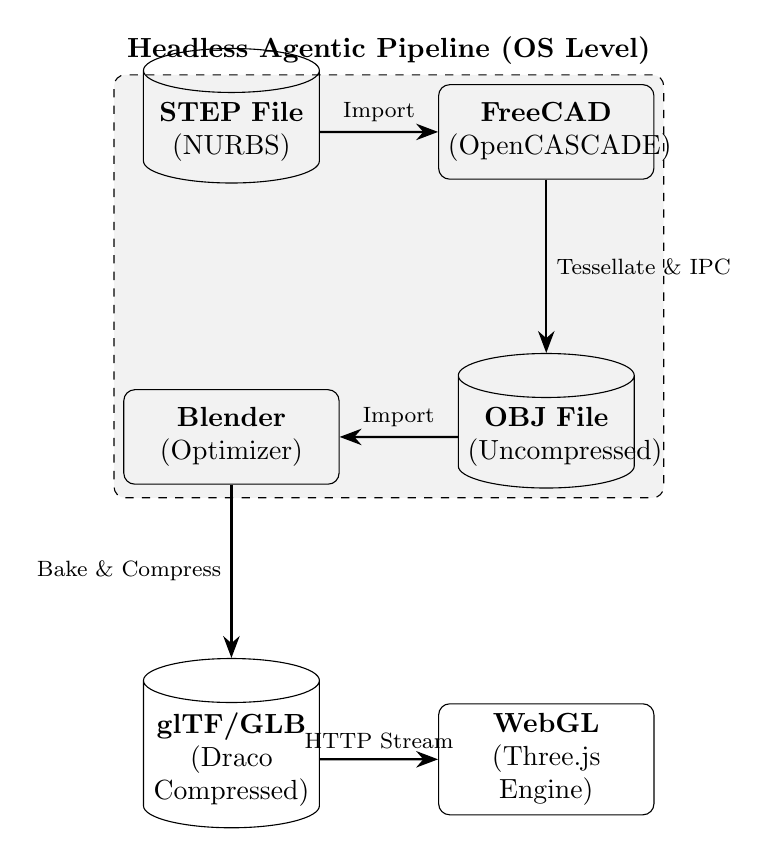
\begin{tikzpicture}[
    node distance=2.2cm and 1.5cm,
    process/.style={rectangle, draw, rounded corners, text width=2.5cm, align=center, minimum height=1.2cm},
    data/.style={cylinder, draw, shape border rotate=90, aspect=0.25, text width=2cm, align=center, minimum height=1.2cm},
    arrow/.style={-{Stealth[scale=1.2]}, thick}
]
    % Nodes
    \node[data] (step) {\textbf{STEP File}\\ (NURBS)};
    \node[process, right=of step] (freecad) {\textbf{FreeCAD}\\ (OpenCASCADE)};
    \node[data, below=of freecad] (obj) {\textbf{OBJ File}\\ (Uncompressed)};
    \node[process, left=of obj] (blender) {\textbf{Blender}\\ (Optimizer)};
    \node[data, below=of blender] (glb) {\textbf{glTF/GLB}\\ (Draco Compressed)};
    \node[process, right=of glb] (webgl) {\textbf{WebGL}\\ (Three.js Engine)};

    % Arrows
    \draw[arrow] (step) -- node[above, font=\footnotesize] {Import} (freecad);
    \draw[arrow] (freecad) -- node[right, font=\footnotesize] {Tessellate \& IPC} (obj);
    \draw[arrow] (obj) -- node[above, font=\footnotesize] {Import} (blender);
    \draw[arrow] (blender) -- node[left, font=\footnotesize] {Bake \& Compress} (glb);
    \draw[arrow] (glb) -- node[above, font=\footnotesize] {HTTP Stream} (webgl);

    % Background Box
    \begin{scope}[on background layer]
        \node[fit=(freecad)(blender)(obj), draw, dashed, fill=gray!10, rounded corners, label=above:\textbf{Headless Agentic Pipeline (OS Level)}] {};
    \end{scope}

\end{tikzpicture}
\caption{The Automated Geometric Translation Pipeline. Data flows from parametric representations to compressed polygonal streams via inter-process communication.}
\label{fig:pipeline}
\end{figure}

This architecture is a form of \textit{store-and-forward} message passing, where the file system acts as the persistent channel buffer between asynchronous producers and consumers. A coordinating agent interfaces with the operating system to spawn a headless instance of the CAD kernel (FreeCAD/OpenCASCADE), which performs tessellation and serializes the intermediate mesh to a shared filesystem medium. The operating system then acts as a message broker, signaling the downstream consumer (Blender) upon write completion to initiate the next processing stage.

\subsection{Semantic Integrity Across the Channel}

During the producer-consumer hand-off, semantic integrity must be preserved. The intermediate Wavefront OBJ format acts as a lingua franca---a plaintext, human-readable serialization of vertices, face indices, and material references. While its verbosity guarantees that no geometry is silently lost in translation, it is enormously inefficient for network transmission; a 10MB CAD assembly routinely expands to a 55MB OBJ file due to the explicit enumeration of every vertex.

This intermediate verbosity is an intentional property of the inter-process contract: it prioritizes semantic fidelity over transmission efficiency, deferring compression to the final serialization stage.

%% ============================================================
\section{Internet Backbones and Geometric Transmission}
\label{sec:backbone}
%% ============================================================

Once the geometry is tessellated and optimized, it must traverse the physical internet to reach a browser client. The internet is not a neutral medium; its topology and bandwidth constraints impose a further geometric lossy compression stage.

\subsection{Network Topology as a Geometric Constraint}

The global internet backbone---a mesh of high-capacity fiber-optic trunk lines interconnecting Tier-1 and Tier-2 autonomous systems---is itself a graph with measurable geometric properties. The path a 3D asset takes from an origin server to a browser endpoint is determined by BGP (Border Gateway Protocol) routing, which optimizes for policy, not latency. Content Delivery Networks (CDNs) partially mitigate this by placing asset replicas at edge nodes topologically close to the consumer.

Nevertheless, fundamental bandwidth constraints remain. A raw 55MB OBJ file representing a single wind turbine at a typical CDN-to-browser throughput of 10 Mbps would require over 40 seconds to transfer---completely untenable for interactive real-time applications managing fleets of agents.

\subsection{The glTF Serialization Standard}

The GL Transmission Format (glTF 2.0) was designed precisely to address this constraint~\cite{b_gltf}. It decouples the structural scene graph (encoded as compact JSON) from the heavy geometric payload (stored as a binary blob, \texttt{.glb}). Additionally, by applying \textit{Draco} mesh compression---a spectral, prediction-based algorithm that exploits the topological regularity of triangle meshes---vertex count and index data are compressed by $60$--$90\%$, reducing our 55MB intermediate representation to a 33MB web-ready asset.

The glTF standard can therefore be understood as a \textit{rate-distortion optimal} codec for 3D geometry: it minimizes transmitted bit-rate while preserving sufficient fidelity for real-time GPU rendering.

%% ============================================================
\section{Conclusion}
\label{sec:conclusion}
%% ============================================================

The deployment of high-fidelity engineering models within browser-based cyber-physical platforms, such as the Sensensble Geometry environment, requires resolving a cascade of geometric and communicative incompatibilities. The parametric precision of NURBS used to design wind turbines and robotic actuators must be sacrificed to the discreteness demanded by GPU rasterization. The semantic integrity of that discretization must be preserved through inter-process message channels. And the resulting payload must be compressed to survive the bandwidth constraints of the global internet backbone.

By treating each stage of this pipeline as a communication channel---with its own fidelity, bandwidth, and encoding standard---we arrive at a unified framework for reasoning about 3D asset delivery. The integration of OpenCASCADE tessellation, OBJ serialization, and glTF/Draco compression successfully collapses the distance between precision engineering environments and distributed web applications. Future work will investigate streaming progressive levels of detail (LOD) for drone swarms, enabling real-time fidelity adaptation based on observed network conditions.

\begin{thebibliography}{00}

\bibitem{b_opencascade} OpenCASCADE Technology, ``OpenCASCADE 3D Modeling Kernel,'' 2024. [Online]. Available: \url{https://www.opencascade.com/}

\bibitem{b_webgl} Khronos Group, ``WebGL Specification,'' 2024. [Online]. Available: \url{https://www.khronos.org/webgl/}

\bibitem{b_gltf} Khronos Group, ``glTF: GL Transmission Format 2.0 Specification,'' 2024. [Online]. Available: \url{https://github.com/KhronosGroup/glTF}

\end{thebibliography}

\end{document}
